\documentclass[compress, aspectratio=169]{beamer}
\usepackage[english]{babel}

\usepackage{amsthm}
\usepackage{mathtools}
\usepackage{physics}
\usepackage{calligra}
\usepackage{csquotes}
\usepackage{tensor}
\usepackage[thicklines]{cancel}
\usepackage{tcolorbox}
\usepackage{pstricks}

\usepackage{multirow}
\usepackage{multicol}
\usepackage{bigdelim}

\usepackage{tabularx}
\usepackage{tikz}
\usepackage{mathtools}
\usepackage{amsmath,amssymb}

%\usepackage[font=footnotesize,labelfont={color=orange,bf}]{caption}
\usepackage{graphicx}

\usepackage[absolute,overlay]{textpos}
%\usepackage[texcoord,grid,gridcolor=red!10,subgridcolor=green!10,gridunit=pt]{eso-pic}

\usepackage{xparse}
\NewDocumentCommand{\framecolorbox}{oommm}
    {% #1 = width (optional)
    % #2 = inner alignment (optional)
    % #3 = frame color
    % #4 = background color
    % #5 = text
    \IfValueTF{#1}
    {%
    \IfValueTF{#2}
     {\fcolorbox{#3}{#4}{\makebox[#1][#2]{#5}}}
     {\fcolorbox{#3}{#4}{\makebox[#1]{#5}}}%
    }
    {\fcolorbox{#3}{#4}{#5}}%
    }

\usepackage[natbib=true,backend=biber,style=apa, sorting=nty, citestyle=authoryear-comp]{biblatex} %Custom bibliography
    \addbibresource{bib.bib} %Load references

\AtBeginBibliography{\footnotesize}

\DeclareMathAlphabet{\mathcalligra}{T1}{calligra}{m}{n}
\DeclareFontShape{T1}{calligra}{m}{n}{<->s*[2.2]callig15}{}
\newcommand{\scriptr}{\mathcalligra{r}\,}
\newcommand{\boldscriptr}{\pmb{\mathcalligra{r}}\,}
\def\rc{\scriptr}
\def\brc{\boldscriptr}
\def\hrc{\hat\brc}
\newcommand{\ie}{\emph{i.e.}} %id est
\newcommand{\eg}{\emph{e.g.}} %exempli gratia
\newcommand{\rtd}[1]{\ensuremath{\left\lfloor #1 \right\rfloor}}
\newcommand{\dirac}[1]{\ensuremath{\delta \left( #1 \right)}}
\newcommand{\diract}[1]{\ensuremath{\delta^3 \left( #1 \right)}}
\newcommand{\e}{\ensuremath{\epsilon_0}}
\newcommand{\m}{\ensuremath{\mu_0}}
\newcommand{\V}{\ensuremath{\mathcal{V}}}
\newcommand{\prnt}[1]{\ensuremath{\left(#1\right)}} %parentheses
\newcommand{\colch}[1]{\ensuremath{\left[#1\right]}} %square brackets
\newcommand{\chave}[1]{\ensuremath{\left\{#1\right\}}}  %curly brackets

\useoutertheme{infolines}
\useinnertheme{rectangles}
\usefonttheme{professionalfonts}


\definecolor{orange}{HTML}{f28165}
\definecolor{gray}{HTML}{303030}
\definecolor{yellow}{HTML}{f0be52}
\definecolor{lightorange}{HTML}{f19e58}
\definecolor{myblue}{cmyk}{1,.72,0,.38}
\definecolor{aliceblue}{rgb}{0.94, 0.97, 1.0}
%\definecolor{mygreen}{RGB}{196, 255, 118}
\definecolor{mygreen}{rgb}{0.53, 0.66, 0.42}
\definecolor{airforceblue}{rgb}{0.36, 0.54, 0.66}

\renewcommand{\CancelColor}{\color{mygreen}}

\makeatletter
\newcommand{\mybox}[1]{%
  \setbox0=\hbox{#1}%
  \setlength{\@tempdima}{\dimexpr\wd0+13pt}%
  \begin{tcolorbox}[colback=mygreen,colframe=mygreen,boxrule=0.5pt,arc=4pt,
      left=6pt,right=6pt,top=6pt,bottom=6pt,boxsep=0pt,width=\@tempdima]
    \textcolor{white}{#1}
  \end{tcolorbox}
}
\makeatother

\usecolortheme[named=mygreen]{structure}
\usecolortheme{sidebartab}
\usecolortheme{orchid}
\usecolortheme{whale}
\setbeamercolor{alerted text}{fg=yellow}
\setbeamercolor{block title alerted}{bg=alerted text.fg!90!black}
\setbeamercolor{block title example}{bg=lightorange!60!black}
\setbeamercolor{background canvas}{bg=gray!80!black}
\setbeamercolor{normal text}{bg=gray!80!black,fg=white}
\setbeamercolor{subsection in head/foot}{bg=white, fg=gray!80!black}


\setbeamertemplate{blocks}[rectangle]
\setbeamercovered{dynamic}

\setbeamertemplate{caption}[numbered]

\setbeamertemplate{section page}
{
	\begin{centering}
		\begin{beamercolorbox}[sep=27pt,center]{part title}
			\usebeamerfont{section title}\insertsection\par
			\usebeamerfont{subsection title}\insertsubsection\par
		\end{beamercolorbox}
	\end{centering}
}

\addtobeamertemplate{navigation symbols}{}{ \hspace{1em}    \usebeamerfont{footline}%
    \insertframenumber / \inserttotalframenumber }
\setbeamertemplate{navigation symbols}{}

%\beamer@compresstrue
\defbeamertemplate*{headline}{smoothbars theme}{%
  \begin{beamercolorbox}[ht=2.125ex,dp=3.150ex]{section in head/foot}
  \insertnavigation{\paperwidth}
  \end{beamercolorbox}%

  \begin{beamercolorbox}[ht=2.125ex,dp=1.125ex,%
  leftskip=.3cm,rightskip=.3cm plus1fil]{subsection in head/foot}
  \usebeamerfont{subsection in head/foot}\insertsubsectionhead
  \end{beamercolorbox}%
}

\setbeamertemplate{subsection page}
{
	\begin{centering}
		\begin{beamercolorbox}[sep=12pt,center]{part title}
			\usebeamerfont{subsection title}\insertsubsection\par
		\end{beamercolorbox}
	\end{centering}
}

\newcommand{\hlight}[1]{\colorbox{violet!50}{#1}}
\newcommand{\hlighta}[1]{\colorbox{red!50}{#1}}

\newcommand{\boxorange}[1]{
\begin{center}
\fcolorbox{orange}{gray}{
\begin{minipage}{0.95\textwidth}
#1
\end{minipage}
}
\end{center}
}

\newcommand{\boxgreen}[1]{
\begin{center}
\fcolorbox{mygreen}{gray!80!black}{
\begin{minipage}{0.95\textwidth}
#1
\end{minipage}
}
\end{center}
}

\newcommand{\boxgrey}[1]{
\begin{center}
\fcolorbox{black!85!white}{lightgray!35!white}{
\begin{minipage}{0.8\textwidth}
#1
\end{minipage}
}
\end{center}
}

\setlength{\abovecaptionskip}{5pt plus 3pt minus 2pt}

% Block colors
\colorlet{orangeTitleBlockColor}{orange}
\colorlet{orangeBlockColor}{orange!25!gray}
\colorlet{greenTitleBlockColor}{mygreen}
\colorlet{greenBlockColor}{mygreen!10!gray}
\colorlet{blockTitleTextColor}{gray!80!black}
\colorlet{blockBodyTextColor}{white}

\setbeamertemplate{blocks}[rectangle]

\setbeamercolor*{block title}{
  fg=blockTitleTextColor,
  bg=greenTitleBlockColor}
\setbeamercolor*{block body}{
  fg=blockBodyTextColor,
  bg=greenBlockColor}
  
\setbeamerfont{block title}{size={}}

\AtBeginEnvironment{block}{%
  \setbeamercolor{itemize item}{fg=greenTitleBlockColor!70}}
  

\title[\cite{eckles2020noise}]{Noise-Induced Randomization \\ in Regression Discontinuity Designs}
%\subtitle{}
\author{Dean Eckles, Nikolaos Ignatiadis, Stefan Wager, Han Wu}
\institute[Sai Zhang]{Presented by: Sai Zhang}
\date{November 18, 2022}

\begin{document}

\bgroup
\setbeamertemplate{navigation symbols}{}
\makeatother
\bgroup

\setbeamertemplate{footline}
        {
      \leavevmode%
      \hbox{%
      \begin{beamercolorbox}[wd=.2\paperwidth,ht=2.25ex,dp=1ex,left]{author in head/foot}%
        \usebeamerfont{author in head/foot}\hspace*{2em} \insertshortinstitute
      \end{beamercolorbox}%
      \begin{beamercolorbox}[wd=.6\paperwidth,ht=2.25ex,dp=1ex,center]{title in head/foot}%
        \usebeamerfont{title in head/foot}\insertshorttitle
      \end{beamercolorbox}%
      \begin{beamercolorbox}[wd=.2\paperwidth,ht=2.25ex,dp=1ex,right]{date in head/foot}%
        \usebeamerfont{date in head/foot}\insertshortdate{}\hspace*{2em}

    %#turning the next line into a comment, erases the frame numbers
        %\insertframenumber{} / \inserttotalframenumber\hspace*{2ex} 

      \end{beamercolorbox}}%
      \vskip0pt%
    }
    
    \frame{\titlepage}
    
    \setbeamertemplate{footline}
        {
      \leavevmode%
      \hbox{%
      \begin{beamercolorbox}[wd=.2\paperwidth,ht=2.25ex,dp=1ex,left]{author in head/foot}%
        \usebeamerfont{author in head/foot}\hspace*{2em}\insertshortinstitute
      \end{beamercolorbox}%
      \begin{beamercolorbox}[wd=.6\paperwidth,ht=2.25ex,dp=1ex,center]{title in head/foot}%
        \usebeamerfont{title in head/foot}\insertshorttitle
      \end{beamercolorbox}%
      \begin{beamercolorbox}[wd=.2\paperwidth,ht=2.25ex,dp=1ex,right]{date in head/foot}%
        \usebeamerfont{date in head/foot}\insertframenumber{}\hspace*{2em}

    %#turning the next line into a comment, erases the frame numbers
        %\insertframenumber{} / \inserttotalframenumber\hspace*{2ex} 

      \end{beamercolorbox}}%
      \vskip0pt%
    }
    \setcounter{framenumber}{0}
    
    \begin{frame}{Outline}
        \tableofcontents
    \end{frame}
    
    \setbeamercovered{invisible}
    \section{Introduction}
\frame{\sectionpage}

\begin{frame}{RD Identification}
    \begin{table}[h!]
    \begin{center}
        \begin{tabular}{ccccccc}
        
        & & \uncover<1->{$\underbrace{Z_i}_\text{running variable}$} & \uncover<3->{$\xRightarrow{W_i=\mathbf{1}\left(\{Z_i\geq {\textcolor<4->{mygreen}{c}}\}\right)}$} & \uncover<2->{$\underbrace{W_i}_\text{treatment}$} & \uncover<5->{$\Rightarrow$} & \uncover<5->{$\underbrace{Y_i}_{\text{outcome}}$}\\
        \uncover<6->{&\\
           \hline
           & \\
            & & test scores & & admission & & outcomes\\}
        \uncover<7->{& & test results && medication && outcomes}
        \end{tabular}
    \end{center}
    \end{table}

\end{frame}

\begin{frame}{RD Identification: Continuity Argument}
    For potential outcomes $\left\{ Y_i(0),Y_i(1) \right\}$: $Y_i=Y_i(W_i)$, a weighted \textcolor{mygreen}{\textbf{causal effect}} can be identified as 
    \begin{align*}
        \tau_c &= \mathbb{E}\left[ Y_i(1)-Y_i(0)\mid Z_i=c \right]\\
        \uncover<2->{&= \textcolor<3->{mygreen}{\lim_{z\downarrow c}}\mathbb{E}\left[Y\mid Z=z\right] - \textcolor<3->{mygreen}{\lim_{z\uparrow c}} \mathbb{E}\left[ Y\mid Z=z \right] }
    \end{align*}
        
    \uncover<3->{
        assuming
        \begin{itemize}
            \item the conditional response functions $\mu_{w}(z)=\mathbb{E}\left[Y(w)\mid Z=z\right]$ are \textcolor{mygreen}{\textbf{\underline{continuous}}}
            \item<4-> $\mu_w(z)$ to have a uniformly \textcolor{mygreen}{\textbf{\underline{bounded 2nd derivative}}} for CIs {\footnotesize\citep{armstrong2018optimal,armstrong2020simple}}
        \end{itemize}
    }

\end{frame}

\begin{frame}{RD Identification: Assumptions of Continuity Argument}
    Assumption: \textcolor{mygreen}{\textbf{\underline{continuous}}} $\mu_{w}(z)=\mathbb{E}\left[Y(w)\mid Z=z\right]$
    \begin{align*}
        \tau_c &= \lim_{z\downarrow c}\mathbb{E}\left[Y\mid Z=z\right] - \lim_{z\uparrow c} \mathbb{E}\left[ Y\mid Z=z \right]
    \end{align*}
    \uncover<1->{
        Where does this continuity come from?
    }

    \vspace*{15pt}
    \uncover<2->{
        \citet{lee2008randomized}: \textcolor{mygreen}{\textbf{\underline{continuous measurement error}}} in the running variable by units
    }

\end{frame}

\begin{frame}{RD Identification: Measurement Error}
    \begin{table}[h!]
    \begin{center}
        \begin{tabular}{ccccccc}
        
       \uncover<1->{$\textcolor<2->{mygreen}{\underbrace{U_i}_{\text{{latent variable}}}}$} & \uncover<2->{$\xRightarrow{Z_i = U_i+ \textcolor<3>{mygreen}{e_i} }$} & $\underbrace{Z_i}_\text{running variable}$ & $\xRightarrow{W_i=\mathbf{1}\left(\{Z_i\geq {\textcolor{mygreen}{c}}\}\right)}$ & $\underbrace{W_i}_\text{treatment}$ & $\Rightarrow$ & $\underbrace{Y_i}_{\text{outcome}}$\\
        &\\
           \hline
           & \\
          \uncover<2->{\textcolor{mygreen}{ability}}  & & test scores & & admission & & outcomes\\
          \uncover<2->{\textcolor{mygreen}{condition}}  & & test results && medication && outcomes
        \end{tabular}
    \end{center}
    \end{table}

    \uncover<3->{
        \vspace*{15pt}
        Why don't we take advantage of the {\textcolor{mygreen}{\textbf{\underline{measurement error}}}} itself for inference?
    }

\end{frame}

\begin{frame}{This Paper}
    \begin{table}[h!]
        \begin{center}
            \begin{tabular}{ccccccc}
          $\underbrace{U_i}_{\text{{latent variable}}}$ & $\xRightarrow{ Z_i\mid U_i\sim \textcolor{mygreen}{p(\cdot\mid U_i)}}$ & $\underbrace{Z_i}_\text{running variable}$ & $\xRightarrow{W_i=\mathbf{1}\left(\{Z_i\geq {\textcolor{mygreen}{c}}\}\right)}$ & $\underbrace{W_i}_\text{treatment}$ & $\Rightarrow$ & $\underbrace{Y_i}_{\text{outcome}}$
            \end{tabular}
        \end{center}
        \end{table}

    Weighted treatment effects can be estimated if the measurement error in $Z_i$
    \begin{itemize}
        \item<2-> has a \textcolor{mygreen}{\textbf{\underline{known distribution}}}
        \item<3-> is \textcolor{mygreen}{\textbf{\underline{conditionally {\footnotesize(on $U_i$)} independent}}} of potential outcomes
    \end{itemize}
    
\end{frame}
    
    \section{Key Argument}
    
    \frame{\sectionpage}

    \begin{frame}{Sharp RD Design with A Noisy Running Variable}
    
        \begin{figure}[h!]
            \centering
            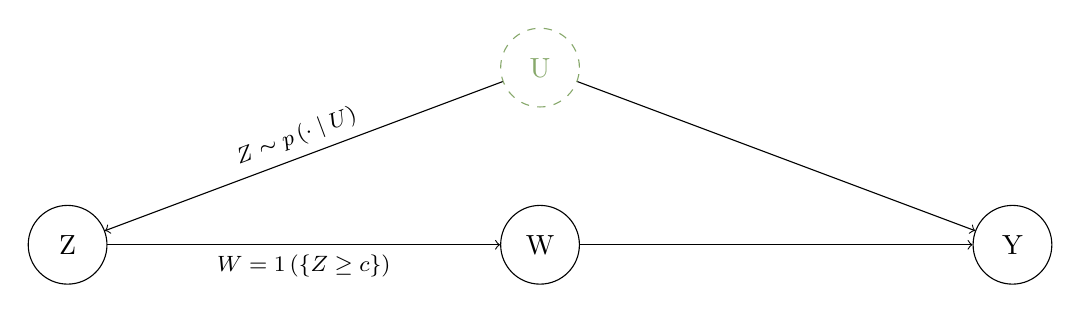
\begin{tikzpicture}[scale=1.5]
        
            \node[circle,draw, minimum size=1cm] (Z) at  (-4,0) {Z};
            \node[circle,draw, minimum size=1cm] (W) at  (0,0) {W};
            \node[circle,draw,dashed,color=mygreen, minimum size=1cm] (U) at (0,1.5) {U};
            \node[circle,draw, minimum size=1cm] (Y) at (4,0) {Y};
            \draw[->] (U) -- (Z) node[midway, font=\footnotesize, sloped, above] { $Z\sim p\left(\cdot\mid U\right)$};
            \draw[->] (Z) -- (W) node[midway, font=\footnotesize, sloped, below] { $W= 1\left( \left\{ Z\geq c \right\} \right)$};
            \draw[->] (W) -- (Y);
            \draw[->] (U) -- (Y);
        \end{tikzpicture}
        \end{figure}

    \end{frame}
    
    \begin{frame}{Sharp RD Design with A Noisy Running Variable}
    
        \begin{figure}[h!]
            \centering
            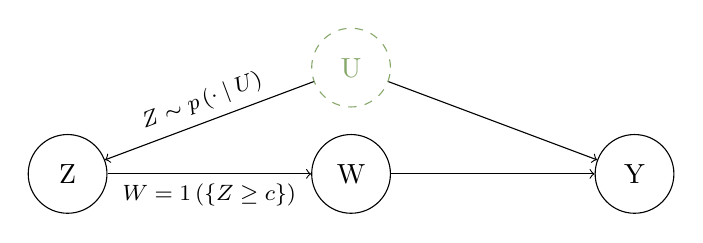
\begin{tikzpicture}[scale=0.9]
        
            \node[circle,draw, minimum size=1cm] (Z) at  (-4,0) {Z};
            \node[circle,draw, minimum size=1cm] (W) at  (0,0) {W};
            \node[circle,draw,dashed,color=mygreen, minimum size=1cm] (U) at (0,1.5) {U};
            \node[circle,draw, minimum size=1cm] (Y) at (4,0) {Y};
            \draw[->] (U) -- (Z) node[midway, font=\footnotesize, sloped, above] { $Z\sim p\left(\cdot\mid U\right)$};
            \draw[->] (Z) -- (W) node[midway, font=\footnotesize, sloped, below] { $W= 1\left( \left\{ Z\geq c \right\} \right)$};
            \draw[->] (W) -- (Y);
            \draw[->] (U) -- (Y);
        \end{tikzpicture}
        \end{figure}

        \only<1->{
            \begin{block}{\textbf{Assumption 1: Sharp RD design}}
                \begin{itemize}
                    \item \underline{\textbf{I.I.D.}} samples $\left\{ Y_i(0),Y_i(1),Z_i \right\}\in\mathbb{R}^3,i=1,\cdots, n$ 
                    \item treatment assignment: $W_i=1\left(\left\{ Z_i\geq c \right\} \right)$, where $c\in \mathbb{R}$ is the \underline{{\textbf{cutoff}}}
                    \item observation: $\left\{ Y_i, Z_i \right\}$ where $Y_i=Y_i(W_i)$
                \end{itemize}
            \end{block}
        }

    \end{frame}
    
    \begin{frame}{Sharp RD Design with A Noisy Running Variable}
    
        \begin{figure}[h!]
            \centering
            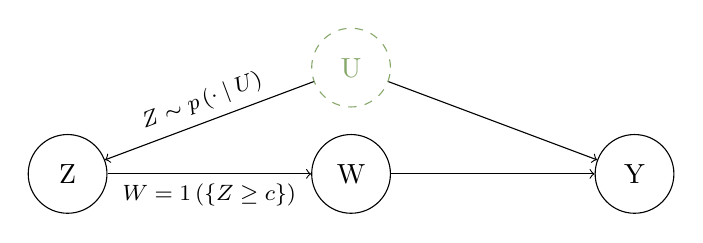
\begin{tikzpicture}[scale=0.9]
        
            \node[circle,draw, minimum size=1cm] (Z) at  (-4,0) {Z};
            \node[circle,draw, minimum size=1cm] (W) at  (0,0) {W};
            \node[circle,draw,dashed,color=mygreen, minimum size=1cm] (U) at (0,1.5) {U};
            \node[circle,draw, minimum size=1cm] (Y) at (4,0) {Y};
            \draw[->] (U) -- (Z) node[midway, font=\footnotesize, sloped, above] { $Z\sim p\left(\cdot\mid U\right)$};
            \draw[->] (Z) -- (W) node[midway, font=\footnotesize, sloped, below] { $W= 1\left( \left\{ Z\geq c \right\} \right)$};
            \draw[->] (W) -- (Y);
            \draw[->] (U) -- (Y);
        \end{tikzpicture}
        \end{figure}

        \begin{block}{\textbf{Assumption 2: Noisy running variable}}
            $$
                Z_i\mid U_i \sim \only<1>{p\left(\cdot \mid U_i\right)} \only<2>{\textcolor{mygreen}{ \mathcal{N}(U_i,\nu^2), \nu>0}} \only<3>{\textcolor{mygreen}{ \mathrm{Binomial}(K,U_i),K\in\mathbb{N}}}
            $$
            where $p(\cdot\mid\cdot)$ is a \textbf{\underline{known}} conditional density w.r.t. to a measure $\lambda$, the latent variable $U_i$ has an \textbf{\underline{unknown}} distribution $G$
            
        \end{block}

    \end{frame}

    \begin{frame}{Sharp RD Design with A Noisy Running Variable}
    
        \begin{figure}[h!]
            \centering
            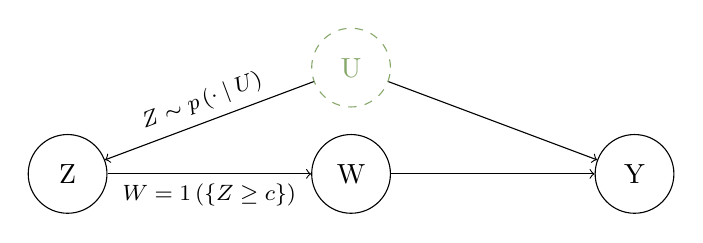
\begin{tikzpicture}[scale=0.9]
        
            \node[circle,draw, minimum size=1cm] (Z) at  (-4,0) {Z};
            \node[circle,draw, minimum size=1cm] (W) at  (0,0) {W};
            \node[circle,draw,dashed,color=mygreen, minimum size=1cm] (U) at (0,1.5) {U};
            \node[circle,draw, minimum size=1cm] (Y) at (4,0) {Y};
            \draw[->] (U) -- (Z) node[midway, font=\footnotesize, sloped, above] { $Z\sim p\left(\cdot\mid U\right)$};
            \draw[->] (Z) -- (W) node[midway, font=\footnotesize, sloped, below] { $W= 1\left( \left\{ Z\geq c \right\} \right)$};
            \draw[->] (W) -- (Y);
            \draw[->] (U) -- (Y);
        \end{tikzpicture}
        \end{figure}

        \only<1->{
            \begin{block}{\textbf{Assumption 3: Exogeneity}}
                $$
                \left[\left\{ Y_{i}\left(0\right),Y_{i}\left(1\right)\right\} \perp Z_{i}\right]\mid U_{i}
                $$
                which implies $\mathbb{E}\left[Y_{i}\mid U_{i},Z_{i}\right]=\alpha_{\left(W_{i}\right)}\left(u\right)$\uncover<2>{, where $\alpha_{\left(w\right)}\left(u\right)=\mathbb{E}\left[Y_{i}\left(w\right)\mid U_{i}=u\right]$ is the \textcolor{mygreen}{\textbf{response functions}} for the potential oucomes conditional on the latent variable $u$}
            \end{block}
        }

    \end{frame}


\begin{frame}{Sharp RD Design with A Noisy Running Variable}
    \begin{columns}[T]
        \begin{column}{0.45\textwidth}
            \begin{figure}[h!]
                \centering
                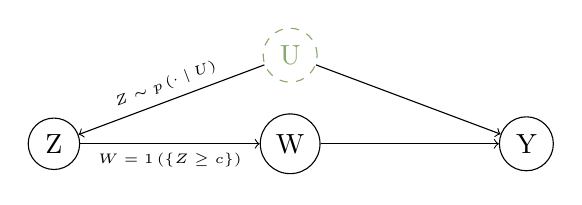
\begin{tikzpicture}[scale=0.75]
            
                \node[circle,draw, minimum size=0.5cm] (Z) at  (-4,0) {Z};
                \node[circle,draw, minimum size=0.5cm] (W) at  (0,0) {W};
                \node[circle,draw,dashed,color=mygreen, minimum size=0.5cm] (U) at (0,1.5) {U};
                \node[circle,draw, minimum size=0.5cm] (Y) at (4,0) {Y};
                \draw[->] (U) -- (Z) node[midway, font=\tiny, sloped, above] { $Z\sim p\left(\cdot\mid U\right)$};
                \draw[->] (Z) -- (W) node[midway, font=\tiny, sloped, below] { $W= 1\left( \left\{ Z\geq c \right\} \right)$};
                \draw[->] (W) -- (Y);
                \draw[->] (U) -- (Y);
            \end{tikzpicture}
            \end{figure}
        \end{column}

        \begin{column}{0.45\textwidth}
            \begin{itemize}
                \item[A1] \textcolor{mygreen}{\underline{\textbf{Sharp}}} RD
                \item[A2] \textcolor{mygreen}{\underline{\textbf{Noisy}}} $Z_i$: $Z_i\mid U_i \sim \only<1>{p\left(\cdot \mid U_i\right)}$
                \item[A3] \textcolor{mygreen}{\underline{\textbf{Exogeneity}}}: $\left[\left\{ Y_{i}\left(0\right),Y_{i}\left(1\right)\right\} \perp Z_{i}\right]\mid U_{i}$
            \end{itemize}
        \end{column}
    \end{columns}

    \uncover<2->{
            \vspace*{15pt}
            \begin{block}{\textbf{Proposition 1}}
                \small
                Let $\gamma_{+}(\cdot),\gamma_{-}(\cdot)$ be measurable functions of $Z$, then under A1-A3:
                \begin{align*}
                    \mathbb{E}\left[\gamma_{+}\left(Z\right)Y\right]&=\mathbb{E}\left[\alpha_{\left(1\right)}\left(U\right)h\left(U,\gamma_{+}\right)\right], & \mathbb{E}\left[\gamma_{-}\left(Z\right)Y\right]&=\mathbb{E}\left[\alpha_{\left(0\right)}\left(U\right)h\left(U,\gamma_{-}\right)\right]
                \end{align*}
                where $h\left(u,\gamma\right)\coloneqq\int\gamma\left(z\right)p\left(z\mid u\right)\mathrm{d}\lambda\left(z\right)$
            \end{block}
        }
    
\end{frame}

\begin{frame}{Sharp RD Design with A Noisy Running Variable}
    \begin{block}{\textbf{Proposition 1}}
        \small
        Let $\gamma_{+}(\cdot),\gamma_{-}(\cdot)$ be measurable functions of $Z$, then under A1-A3:
        \begin{align*}
            \mathbb{E}\left[\gamma_{+}\left(Z\right)Y\right]&=\mathbb{E}\left[\alpha_{\left(1\right)}\left(U\right)h\left(U,\gamma_{+}\right)\right], & \mathbb{E}\left[\gamma_{-}\left(Z\right)Y\right]&=\mathbb{E}\left[\alpha_{\left(0\right)}\left(U\right)h\left(U,\gamma_{-}\right)\right]
        \end{align*}
        where $h\left(u,\gamma\right)\coloneqq\int\gamma\left(z\right)p\left(z\mid u\right)\mathrm{d}\lambda\left(z\right)$
    \end{block}

    \uncover<2->{
        \vspace*{5pt}
        \begin{itemize}
            \item<2-> $\mathbb{E}\left[Y^2\right], \mathbb{E}\left[\gamma_{-}\left(Z\right)^{2}\right],\mathbb{E}\left[\gamma_{+}\left(Z\right)^{2}\right]<\infty$
            \item<3-> $\gamma_{+}(\cdot),\gamma_-(\cdot)$ are weighting functions s.t.
            \begin{itemize}
                \item<4->[-] $\gamma_{+}\left(z\right)=0$ for $z<c$: assign non-zero weights only to \textcolor{mygreen}{\textbf{treated}} units
                \item<5->[-] $\gamma_{-}\left(z\right)=0$ for $z\geq c$: assign non-zero weights only to \textcolor{mygreen}{\textbf{control}} units
            \end{itemize}
        \end{itemize}
    }

    \uncover<6->{
        \vspace*{5pt}
        To achieve balance in the \textcolor{mygreen}{\textbf{latent variable}}: $h(\cdot,\gamma_+)\approx h(\cdot,\gamma_-)$
        \vspace*{10pt}
    }
    
    
\end{frame}
    
    \section{Estimation}

 \frame{\sectionpage}

    \begin{frame}{Estimation of Weighted Treatment Effects}
        \begin{block}{\textbf{Proposition 1}}
            \small
            Let $\gamma_{+}(\cdot),\gamma_{-}(\cdot)$ be measurable functions of $Z$, then under A1-A3:
            \begin{align*}
                \mathbb{E}\left[\gamma_{+}\left(Z\right)Y\right]&=\mathbb{E}\left[\alpha_{\left(1\right)}\left(U\right)h\left(U,\gamma_{+}\right)\right], & \mathbb{E}\left[\gamma_{-}\left(Z\right)Y\right]&=\mathbb{E}\left[\alpha_{\left(0\right)}\left(U\right)h\left(U,\gamma_{-}\right)\right]
            \end{align*}
            where $h\left(u,\gamma\right)\coloneqq\int\gamma\left(z\right)p\left(z\mid u\right)\mathrm{d}\lambda\left(z\right)$, $\alpha_{\left(w\right)}\left(u\right)=\mathbb{E}\left[Y_{i}\left(w\right)\mid U_{i}=u\right]$
        \end{block}

        


    \end{frame}


    \section{CIs}

 \frame{\sectionpage}

 \begin{frame}{Asymptotic Normality}
    \begin{align*}
        \hat{\tau} =& \frac{\sum_i \gamma_+\left(Z_i\right)Y_i}{\sum_i {\gamma_+\left(Z_i\right)} } - \frac{\sum_i \gamma_-\left(Z_i\right)Y_i}{\sum_i {\gamma_-\left(Z_i\right)} }\\
        \hat{\tau}_{\gamma}\xrightarrow{p}\theta_{\gamma}= & \frac{\mathbb{E}\left[\alpha_{\left(1\right)}\left(U\right)h\left(U,\gamma_{+}\right)\right]}{\mathbb{E}\left[h\left(U,\gamma_{+}\right)\right]}-\frac{\mathbb{E}\left[\alpha_{\left(0\right)}\left(U\right)h\left(U,\gamma_{-}\right)\right]}{\mathbb{E}\left[h\left(U,\gamma_{-}\right)\right]} \\
        a\mathrm{Bias}=\theta_{\gamma}-\tau_{w}= & \underbrace{\int\left(\frac{h\left(u,\gamma_{+}\right)}{\mathbb{E}_{G}\left[h\left(U,\gamma_{+}\right)\right]}-\frac{h\left(u,\gamma_{-}\right)}{\mathbb{E}_{G}\left[h\left(U,\gamma_{-}\right)\right]}\right)\alpha_{\left(0\right)}\left(u\right)\mathrm{d}G\left(u\right)}_{\text{Confounding bias}} \\
         & +\underbrace{\int\left(\frac{h\left(u,\gamma_{+}\right)}{\mathbb{E}_{G}\left[h\left(U,\gamma_{+}\right)\right]}-\frac{w\left(u\right)}{\mathbb{E}_{G}\left[w\left(U\right)\right]}\right)\tau\left(u\right)\mathrm{d}G\left(u\right)}_{\text{CATE heterogeneity bias}}
    \end{align*}        
 \end{frame}

 \begin{frame}{Asymptotic Normality}
    \begin{block}{\textbf{Theorem: Asymptotic Normality of $\hat{\tau}$}}
        \small
        Suppose the sequence of weighting kernels $\gamma_{+}^{\left(n\right)}$ and $\gamma_{-}^{\left(n\right)}$ is deterministic, and  $\exists\beta\in\left(0,\frac{1}{2}\right), C,C'>0$ s.t. $\forall n$ large enough:
        \begin{align*}
            \sup_{z}\left|\gamma_{\diamond}^{\left(n\right)}\left(z\right)\right|&<Cn^{\beta}\left[\gamma_{\diamond}^{\left(n\right)}\left(Z_{i}\right)\right] & \sup_{u}\left|h\left(u,\gamma_{\diamond}^{\left(n\right)}\right)\right|&<C'\mathbb{E}\left[\gamma_{\diamond}^{\left(n\right)}\left(Z_{i}\right)\right], & \diamond&=\left\{ +,-\right\} 
        \end{align*}
        where $h\left(u,\gamma\right)\coloneqq\int\gamma\left(z\right)p\left(z\mid u\right)\mathrm{d}\lambda\left(z\right)$, $\alpha_{\left(w\right)}\left(u\right)=\mathbb{E}\left[Y_{i}\left(w\right)\mid U_{i}=u\right]$
    \end{block}
    
 \end{frame}

    \section{Applications}

 \frame{\sectionpage}

\begin{frame}{Design Estimators}
    The goal: Make the confidence intervals \textcolor{mygreen}{\textbf{shorter}}
    \begin{align*}
        \hat{\tau}_{\gamma}&\pm l_{\alpha}, &l_{\alpha}&=\min\left\{ l:\mathbf{P}\left[\left|b+n^{-\frac{1}{2}}\hat{V}_{\gamma}^{\frac{1}{2}}\tilde{Z}\right|\leq l\right]\geq1-\alpha,\forall\left|b\right|\leq\hat{B}_{\gamma,M}\right\} 
    \end{align*}

    by minimizing the worst-case MSE of
    $$
    \hat{\tau}= \hat{\mu}_{\gamma,+}- \hat{\mu}_{\gamma,-}=\frac{\sum_{i}\gamma_{+}\left(Z_{i}\right)Y_{i}}{\sum_{i}\gamma_{+}\left(Z_{i}\right)} - \frac{\sum_{i}\gamma_{-}\left(Z_{i}\right)Y_{i}}{\sum_{i}\gamma_{-}\left(Z_{i}\right)}
    $$
\end{frame}

\begin{frame}{Design Estimators: Quadratic Programming}
    Solve
    $$
    \min_{\gamma_{\pm}\left(\cdot\right)}\frac{1}{n}\left( \textcolor<2>{mygreen}{\int\gamma_{-}^{2}\left(z\right)\mathrm{d}\bar{F}\left(z\right)+\int\gamma_{+}^{2}\left(z\right)\mathrm{d}\bar{F}\left(z\right)} \right)+\left(t_{1}+t_{2}\right)^{2}
    $$
    s.t.
    {\small
        \begin{align*}
        \left|h\left(u,\gamma_{+}\right)-h\left(u,\gamma_{-}\right)\right| & \leq t_{1}, & \forall u &  & \uncover<3->{\text{confounding bias}}\\
        M\left|h\left(u,\gamma_{\diamond}\right)-\bar{w}\left(u\right)\right| & \leq t_{2}, & \forall u,\diamond\in\left\{ \pm\right\}  &  & \uncover<3->{\text{CATE-hetrogeneity bias}}\\
        \int\gamma_{+}\left(z\right)\mathrm{d}\bar{F}\left(z\right)=\int\gamma_{-}\left(z\right)\mathrm{d}\bar{F}\left(z\right) & =1 &  &  & \uncover<4->{\text{normalization constraint}} \\
        \gamma_{-}\left(z\right) & =0, & z\geq c &  & \uncover<4->{\text{Sharp RD}} \\
        \gamma_{+}\left(z\right) & =0, & z<c\\
        \left|\gamma_{\diamond}\left(z\right)\right| & \leq Cn^{\beta}, & \forall z,\diamond\in\left\{ \pm\right\}  &  & \uncover<5->{\text{no observation is given excessive influence}}
    \end{align*}}
        
\end{frame}

\begin{frame}{Design Estimators: Quadratic Programming}
    Solve
    $$
    \min_{\gamma_{\pm}\left(\cdot\right)}\frac{1}{n}\left( {\int\gamma_{-}^{2}\left(z\right)\mathrm{d}\textcolor<2>{mygreen}{\bar{F}}\left(z\right)+\int\gamma_{+}^{2}\left(z\right)\mathrm{d}\textcolor<2>{mygreen}{\bar{F}}\left(z\right)} \right)+\left(t_{1}+t_{2}\right)^{2}
    $$
    s.t.
    {\small
        \begin{align*}
        M\left|h\left(u,\gamma_{\diamond}\right)-\textcolor<2>{mygreen}{\bar{w}}\left(u\right)\right| & \leq t_{2}, & \forall u,\diamond\in\left\{ \pm\right\}  &  & {\text{CATE-hetrogeneity bias}}\\
        \int\gamma_{+}\left(z\right)\mathrm{d}\textcolor<2>{mygreen}{\bar{F}}\left(z\right)=\int\gamma_{-}\left(z\right)\mathrm{d}\textcolor<2>{mygreen}{\bar{F}}\left(z\right) & =1 &  &  & {\text{normalization constraint}}
    \end{align*}}

    \uncover<2->{
        \small
        \begin{align*}
            &\bar{F}(\cdot): &F_{G}\left(t\right) &= \int\mathbf{1}\left(\left\{ z\leq t\right\} \right)\int p\left(z\mid u\right)\mathrm{d}G\left(u\right)\mathrm{d}\lambda\left(z\right) \\
            &\bar{w}(\cdot): &\tau_{w}&= \int\frac{w\left(u\right)}{\mathbb{E}_{G}\left[w\left(U\right)\right]}\tau\left(u\right)\mathrm{d}G\left(u\right)
        \end{align*}
    }
\end{frame}

\begin{frame}{Design Estimators: Quadratic Programming}

    {
        \small
        \begin{align*}
            &\bar{F}(\cdot): &F_{G}\left(t\right) &= \int\mathbf{1}\left(\left\{ z\leq t\right\} \right)\int p\left(z\mid u\right)\mathrm{d}G\left(u\right)\mathrm{d}\lambda\left(z\right) \\
            &\bar{w}(\cdot): &\tau_{w}&= \int\frac{w\left(u\right)}{\mathbb{E}_{G}\left[w\left(U\right)\right]}\tau\left(u\right)\mathrm{d}G\left(u\right)
        \end{align*}
    }

    \begin{itemize}
        \item $\bar{F}\left(\cdot\right)$ assigns non-trivial mass to $\left[c,\infty\right)$ and $\bar{w}(\cdot)$ is bounded: $\exists k>1$ s.t.
        $$\mathbb{P}\left[\frac{1}{k}<\bar{F}\left(\left[c,\infty\right)\right)<1-\frac{1}{k},\sup_{u}\left|\bar{w}\left(u\right)\right|<k\right]\xrightarrow{n\rightarrow\infty}1$$
        \item $\int\gamma_{\diamond}^{\left(n\right)}\left(z\right)\mathrm{d}F\left(z\right)$ is asymptotically lower bounded by a strictly positive number: $$\exists\delta>0\text{ s.t. } \mathbb{P}\left[\int\gamma_{\diamond}^{\left(n\right)}\left(z\right)\mathrm{d}F\left(z\right)>\delta\right]\xrightarrow{n\rightarrow\infty}1$$
    \end{itemize}
    
\end{frame}

\begin{frame}{Design Estimators: Quadratic Programming}
    $$
    \begin{aligned}
        \frac{1}{k}<\bar{F}\left(\left[c,\infty\right)\right)<1-\frac{1}{k},\sup_{u}\left|\bar{w}\left(u\right)\right| &<k\\
        \int\gamma_{\diamond}^{\left(n\right)}\left(z\right)\mathrm{d}F\left(z\right) &>\delta
    \end{aligned}\Rightarrow 
    \begin{aligned}
        &\sup_{z}\left|\gamma_{\diamond}^{\left(n\right)}\left(z\right)\right| <Cn^{\beta}  \mathbb{E} \left[\gamma_{\diamond}^{\left(n\right)}\left(Z_{i}\right)\right]\\
        &\sup_{u}\left|h\left(u,\gamma_{\diamond}^{\left(n\right)}\right)\right| <C'\mathbb{E}\left[\gamma_{\diamond}^{\left(n\right)}\left(Z_{i}\right)\right]
    \end{aligned}\uncover<2>{\Rightarrow}
    $$

    \only<2>{\begin{block}{\textbf{Theorem: Asymptotic Normality of $\hat{\tau}$}}
        \small
        Suppose the sequence of weighting kernels $\gamma_{+}^{\left(n\right)}$ and $\gamma_{-}^{\left(n\right)}$ is deterministic, and  $\exists\beta\in\left(0,\frac{1}{2}\right), C,C'>0$ s.t. $\forall n$ large enough: $\sup_{z}\left|\gamma_{\diamond}^{\left(n\right)}\left(z\right)\right| <Cn^{\beta}  \mathbb{E} \left[\gamma_{\diamond}^{\left(n\right)}\left(Z_{i}\right)\right]$, $\sup_{u}\left|h\left(u,\gamma_{\diamond}^{\left(n\right)}\right)\right| <C'\mathbb{E}\left[\gamma_{\diamond}^{\left(n\right)}\left(Z_{i}\right)\right]$ where $\diamond=\left\{ +,-\right\}$
        Then 
        $$
        \frac{\sqrt{n}\left(\hat{\tau}_{\gamma}-\theta_{\gamma}\right)}{\sqrt{V_{\gamma}}}\xrightarrow{d}\mathcal{N}\left(0,1\right)
        $$
    \end{block}}
\end{frame}

\begin{frame}{Design Estimators: Procedure}

    \begin{itemize}
        \item<1-> \textcolor{mygreen}{\textbf{Input:}}
        \begin{itemize}
            \item[-] samples $ \left\{ Z_{i},Y_{i},W_{i}\right\} $ and cutoff $c$
            \item[-] sensitivity model $\mathcal{T}_{M}$, estimand of interest $\tau_{w}$
            \item[-] nominal significance level $\alpha$ 
        \end{itemize}

        \item<2-> \textcolor{mygreen}{\textbf{Procedure:}}
        \begin{itemize}
            \item[S1] guess/estimate $\bar{F}\left(\cdot\right)$ and $\bar{w}\left(\cdot\right)$ via nonparametric maximum likelihood
            \item[S2] solve the minimax program, get $\gamma_{+},\gamma_{-}$ 
            \item[S3] form the point estimate $\hat{\tau}_{\gamma}$ and its variance $\hat{V}_{\gamma}$
            \item[S4] estimate the worst-case bias $\hat{B}_{\gamma}=\sup\left\{ \left|\mathrm{Bias}\left[\gamma_{\pm},\tau_{w};\alpha_{0}\left(\cdot\right),\tau\left(\cdot\right),G\right]\right|:G\in\mathcal{G}_{n},\alpha_{\left(0\right)}\left(\cdot\right)\in\left[0,1\right],\tau\left(\cdot\right)\in\mathcal{T}_{M}\right\} $
            \item[S5] form the bias-aware CIs at level $\alpha$ as $\hat{\tau}_{\gamma}\pm l_{\alpha},l_{\alpha}=\min\left\{ l:\mathbf{P}\left[\left|b+n^{-\frac{1}{2}}\hat{V}_{\gamma}^{\frac{1}{2}}\tilde{Z}\right|\leq l\right]\geq1-\alpha,\forall\left|b\right|\leq\hat{B}_{\gamma,M}\right\} $
        \end{itemize}
    \end{itemize}
    
\end{frame}

    \section{Discussion}
    
    \frame{\sectionpage}

    \begin{frame}{Noise-Induced RD vs Continuity-Based RD}

    \end{frame}
    
    \begin{frame}{Literature: Concerns addressed}
        
    \end{frame}

    

\section*{References}
\begin{frame}[allowframebreaks]{References}
    \printbibliography[heading=none]
\end{frame}
    
\part{}
    \begin{frame}[plain,c]
    \begin{center}
       \Huge
        \textcolor{mygreen}{Thank you!} 
        
    \end{center}
    \end{frame}
\end{document}
